\section{Hierarchisches Modell für korrelierte Felder}\label{k4.2.hiera}
\sectionauthor{Natalie Teplitska, Clemens Ljungh, Constantin Burmeister}
Im Folgenden wird der Prior $P(s)$ für die Radioastronomie und Tomographie diskutiert. In unserem Modell müssen wir glatte Signale $s$ darstellen können. Eine besonders einfache Art,, diese zu formulieren ist über einen hierarchischen Aufbau. Zu diesem Zweck wird im Folgenden die Python Bibliothek \emph{NIFTy8} benutzt.

Ziel eines bildgebenden Verfahrens ist die Bestimmung von $s$. Dies kann bei der Radioastronomie die Helligkeit des Himmels oder bei der CT die Dichte des untersuchten Objektes sein. Da weder Helligkeit noch Dichte negativ sein kann, setzen wir $s \geq 0$ voraus. Damit lässt sich eine Normalverteilung für $P(s)$ bereits ausschließen, da eine solche über ganz $\mathbb{R}$ definiert wäre. Außerdem wird angenommen, dass die einzelnen Bildpunkte miteinander korreliert sind, also voneinander abhängen. Ist zum Beispiel ein Pixel dunkel, so ist es unwahrscheinlich, dass sich in direkter Nähe dazu helle Pixel befinden. In unserem Fall gilt, dass die Abhängigkeit zunimmt, je kleiner dar Abstand zwischen zwei Pixeln ist. Daraus ergibt sich eine schwierig darzustellende Kovarianzmatrix, die die Korrelation der Pixel zueinander codiert.

Wir reduzieren die Komplexität von $s$, indem wir eine weitere hierarchische Stufe ergänzen. Als Zufallsvariable wird statt $s$ nun $\xi$ verwendet, welches mit $P(\xi) = \mathbb{G}(\xi, \mathds{1})$ standard-nor\-mal\-ver\-teilt ist.

Unsere Aufgabe bestand nun darin, eine Funktion $f$ so zu definieren und zu implementieren, sodass $P(f(\xi)) d \xi = P(s) ds$. Die Schwierigkeit besteht in der Codierung der Kovarianzmatrix in $f$.

Die \emph{Cholesky-Zerlegung} stellt eine Möglichkeit dar, ein solches $f$ zu erzeugen, wobei nur eine Dreiecksmatrix mit halb so vielen Einträgen gespeichert werden muss. Anschaulich gesprochen ziehen wir aus $s$ die Wurzel, sodass $S=A A^{\dagger}$. Auf diese Weise lässt sich eine Funktion definieren, die aus zufälligen Zahlen $\xi$ den Prior über $s$ berechnet: $s = f(\xi) = A \cdot \xi$. Allerdings ist der Speicherverbrauch der Dreiecksmatrix für $\mathcal{O}(100 000)$ Datenpunkte immer noch enorm.

Einen alternativen Ansatz stellt das \emph{Wiener-Chintchin-Theorem} dar. Hier wird die Annahme getroffen, dass die Kovarianz zwischen den Pixeln nur von deren Entfernung, nicht jedoch von deren Position abhängt. Dabei gilt
\begin{eqnarray}
S= \mathcal{F}^{\dagger} diag(p(|k|)) \mathcal{F} \ .
\end{eqnarray}
Wir haben damit erfolgreich die Kovarianzmatrix in eine diagonale Form gebracht: das Powerspektrum $diag(p(|k|))$. Mit der Hartley-Transformation \footnote{Variante der Fourier-Transformation, welche Real- und Imaginärteil im reellen Raum verrechnet} übersetzen wir vom Raum des Powerspektrums zum Raum der Kovarianzmatrix.

Bisher haben wir mit einer vorgegebenen Kovarianz $S$ gearbeitet. Um aus Daten lernen zu können, wollen wir uns allerdings nicht auf eine bestimmte Kovarianzmatrix festlegen. Die Berechnung des Posteriors gestaltet sich wesentlich einfacher, wenn das Powerspektrum über eine Menge von Parametern definiert wird. Diese können jeweils mit Bayes (siehe \cref{k4.2.bayes}) immer weiter angepasst werden. Für unseren Fall arbeiteten wir mit drei Parametern (siehe \cref{k4.2.power-function.img}).
\begin{figure}[h] 
    \centering
    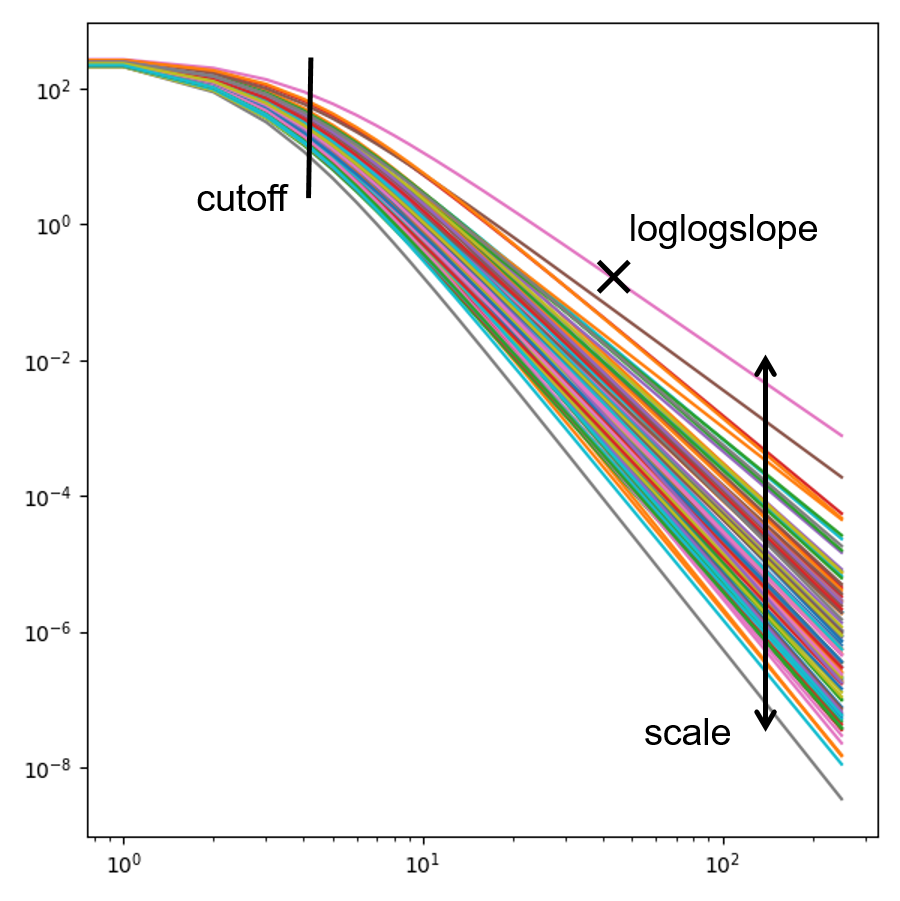
\includegraphics[width=0.4\textwidth]{k4.2/power_function_bearbeitet.png}
    \caption{100 beispielhafte power functions und ihre Parameter}
    \label{k4.2.power-function.img}
\end{figure}
\begin{itemize}
    \item Der Parameter \emph{scale} steht für die Standardabweichung des Powerspektrums und beschreibt somit, wie stark es variieren kann.
    \item Wir gehen von einer Funktion aus, die rechts von einem bestimmten Punkt eine Form annimmt, welche einem power-law folgt. Diesen Punkt bezeichnet man als \emph{cutoff}.
    \item Schließlich bezeichnet \emph{loglogslope} die Steigung der Funktion in dem Intervall nach dem cutoff.
\end{itemize}
Alle drei Parameter werden über je zwei Zahlenwerte definiert: den Mittelwert der Erwartungen und seine vermutete Varianz. Im Grunde genommen arbeiten wir also mit sechs Zahlenwerten, die unter Einbezug von Daten immer weiter angepasst werden können.

Damit haben wir es geschafft, einen Prior für $s$ mittels a priori sehr einfach verteilten Zufallszahlen zu generieren, der ein Lernen aus Daten mit kleinstmöglichem Rechen- und Speicheraufwand ermöglicht.
